\documentclass[10pt,twocolumn]{article}
\usepackage[a4paper,margin=1.6cm,columnsep=0.6cm]{geometry}
\usepackage{amsmath,booktabs,graphicx}
\usepackage[hidelinks]{hyperref}
\usepackage[small,compact]{titlesec}
\usepackage[font=small,skip=3pt]{caption}
\setlength{\parskip}{0pt}
\graphicspath{{../}}

\title{\vspace{-1.2cm}\textbf{DustWise: Water-Aware Solar Panel Cleaning in the Thar Desert with Reinforcement Learning}\vspace{-0.3cm}}
\author{\small
Ramcharan (B23CI1032)\\
\small GitHub: \url{https://github.com/RamcharanRajpurohit/dustwise}}
\date{\vspace{-0.9cm}}

\begin{document}
\maketitle

\section{Problem}
Desert dust cuts the output of Rajasthan's solar plants by up to 30\%, but cleaning costs labour and, for a water wash, scarce trucked water. Light rain makes things worse: it cements loose dust so that only water removes it, while heavy rain cleans panels for free. A plant operator must decide every day which part of the plant to clean and how. We model a 10\,MWp plant in Jaisalmer as 10 blocks of 1\,MWp (1,820 modules each), with one cleaning crew that treats one block per day, and train an RL agent to make that daily decision. The environment is driven by real data for Jaisalmer (26.91\,N, 70.91\,E), 2022-08 to 2025: ERA5 irradiance and rain, CAMS dust, and archived day-ahead forecasts, all from Open-Meteo.

\section{RL formulation}
\textbf{State $\mathcal{S}$ (26-dim, continuous).} For each block $i$: loose soiling loss $\ell_i$ and cemented loss $c_i$ (scaled $\times10$); tank level $w/10^4$\,L; the day-ahead forecast of irradiance $\hat H_t/7$ and rain $\min(\hat R_t,12)/6$; today's CAMS dust $D_t/9500$; and the season, $(1+\sin\phi_t)/2$ and $(1+\cos\phi_t)/2$ with $\phi_t=2\pi\,\mathrm{doy}/365.25$.

\textbf{Action $\mathcal{A}$ (discrete, 21).} $a=0$ idle; $a=1..10$ dry-brush block $i$; $a=11..20$ water-wash block $i$. Washes are masked out when $w<3640$\,L (one wash).

\textbf{Dynamics (one step = one day).} In the morning a brush sets $\ell_i\leftarrow0.1\,\ell_i$; a wash sets $\ell_i=c_i=0$ and $w\leftarrow w-3640$. The plant then generates with the \emph{actual} irradiance $H_t$. Afterwards the actual rain $R_t$ updates the dust: if $R_t\ge6$\,mm all blocks are clean; if $0<R_t<6$, $c_i\leftarrow c_i+\ell_i$, $\ell_i\leftarrow0$. New dust settles as $\ell_i\leftarrow\ell_i+0.004\,D_t/\bar D$ ($\bar D=950\,\mu$g/m$^3$), and the tank refills by 1,000\,L/day up to 10,000\,L.

\textbf{Reward $\mathcal{R}$.} The negative daily cost in units of $10^4$ INR:
\begin{align*}
r_t=-10^{-4}\Big(&\tau P\,\mathrm{PR}\,H_t\textstyle\sum_i\min(\ell_i+c_i,\,0.3)\\
&+364\,[a\neq0]+874\,[a>10]\Big)
\end{align*}
where the first term is lost revenue and the others labour and water,
tariff $\tau=2.5$ INR/kWh, $P=1000$\,kWp and $\mathrm{PR}=0.78$. Labour is 0.20 INR and water 2\,L at 0.24 INR/L per module. The agent therefore trades certain cleaning costs now against uncertain soiling losses that may be erased by rain.

\textbf{Constants} come from published sources: soiling 0.37\%/day measured in Gandhinagar~\cite{valerino}, the 6\,mm rain threshold and 30\% cap of the Kimber model~\cite{pvlib}, rain cementation~\cite{valerino,renene}, and Indian tender and auction prices for labour, water and tariff (listed in the README).

\textbf{Episodes} are 90 random consecutive days from 2022-08 to 2024. 2025 is the held-out test year, played as one 364-day episode. Archived forecasts exist only from 2024-01-20, so earlier training days use the observed weather as the forecast; on 2024--25 the real forecast has irradiance correlation 0.89 (nRMSE 13\%) and caught only 14 of 25 heavy-rain days with 18 false alarms. The agent must act under genuine forecast uncertainty.

\section{Algorithms and baselines}
\textbf{Baselines.} No cleaning; daily rotation with a brush; daily rotation with a wash; and \emph{greedy}: brush the dustiest block unless heavy rain is forecast. Greedy is the strongest rule.

\textbf{Algorithms.} All use Stable-Baselines3~\cite{sb3}, a 128$\times$128 MLP and $\gamma=0.9$ (soiling effects decay within days). We compare DQN (3-step returns), QR-DQN, PPO, A2C and MaskablePPO~\cite{maskppo}, each with 3 seeds and 500k steps. MaskablePPO receives the tank mask so it never wastes a crew-day on an impossible wash.

\textbf{Final agent (v3).} We held out 2024 as a validation year (training on 2022--23) and tested additions to MaskablePPO one at a time. A season input and an entropy bonus of 0.01 helped (2024 cost 19.16$\to$17.55 lakh INR); PPO settings from An~\cite{an} and 2--3-day rain forecasts (suggested by Terhag et al.~\cite{terhag}) helped less. The final agent retrains on 2022--24 for 1M steps.

\section{Results on unseen 2025}

\begin{table}[h]
\centering\footnotesize\setlength{\tabcolsep}{4pt}
\begin{tabular}{lccc}
\toprule
Policy & Cost (lakh INR) & Lost MWh & Water kL\\
\midrule
No cleaning$^\dagger$ & 47.79 & 1912 & 0\\
Rotation wash$^\dagger$ & 25.29 & 961 & 371\\
Rotation brush$^\dagger$ & 19.62 & 732 & 0\\
Greedy brush & 19.63 & 735 & 0\\
DQN & 17.30$\pm$0.77 & 632 & 220\\
QR-DQN & 18.80$\pm$0.97 & 691 & 203\\
PPO & 15.39$\pm$0.23 & 567 & 165\\
A2C & 16.22$\pm$0.24 & 604 & 131\\
MaskablePPO & 14.18$\pm$0.19 & 513 & 204\\
\textbf{v3 MaskablePPO} & \textbf{13.00$\pm$0.04} & \textbf{467} & \textbf{175}\\
\bottomrule
\end{tabular}
\caption{Total 2025 cost with real forecasts, mean $\pm$ std over 3 seeds. $^\dagger$Forecast-independent rules (from v1, perfect forecast).}
\end{table}

\begin{figure*}[t]
\centering
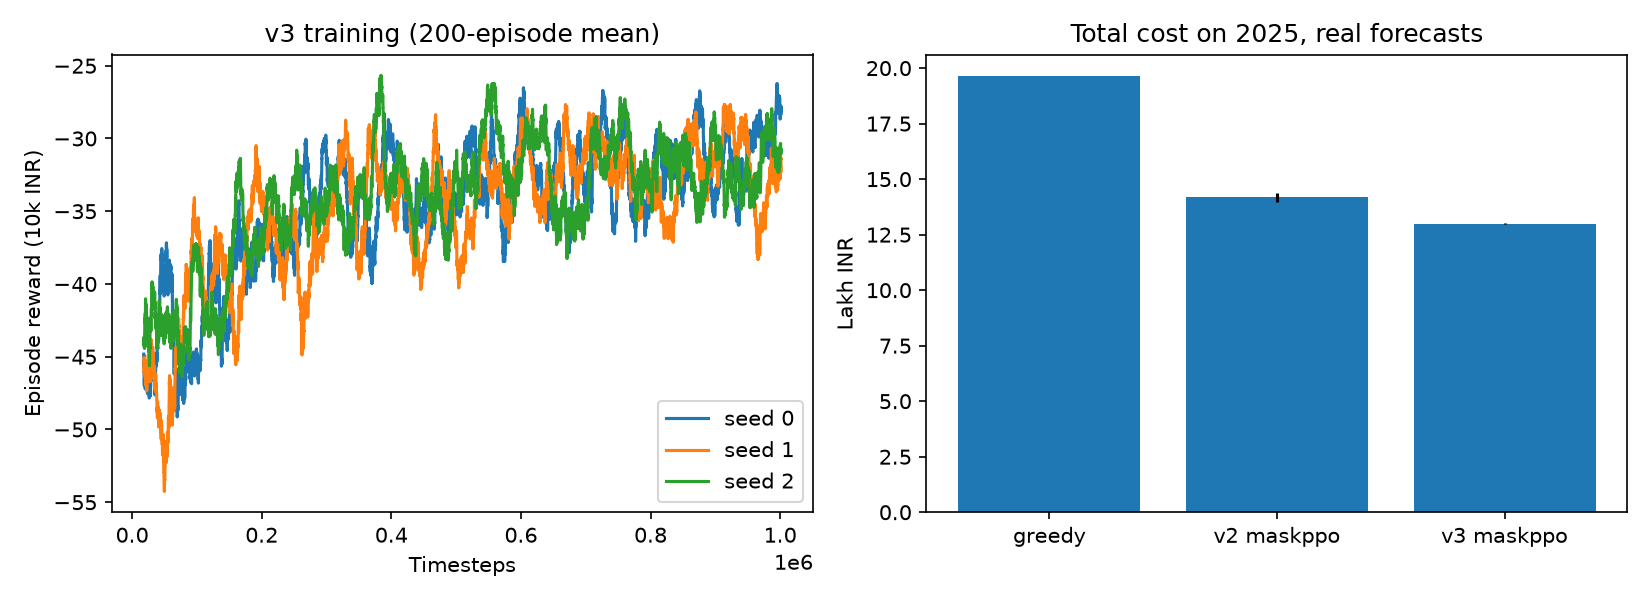
\includegraphics[width=0.49\textwidth]{v3/results_v3.png}\hfill
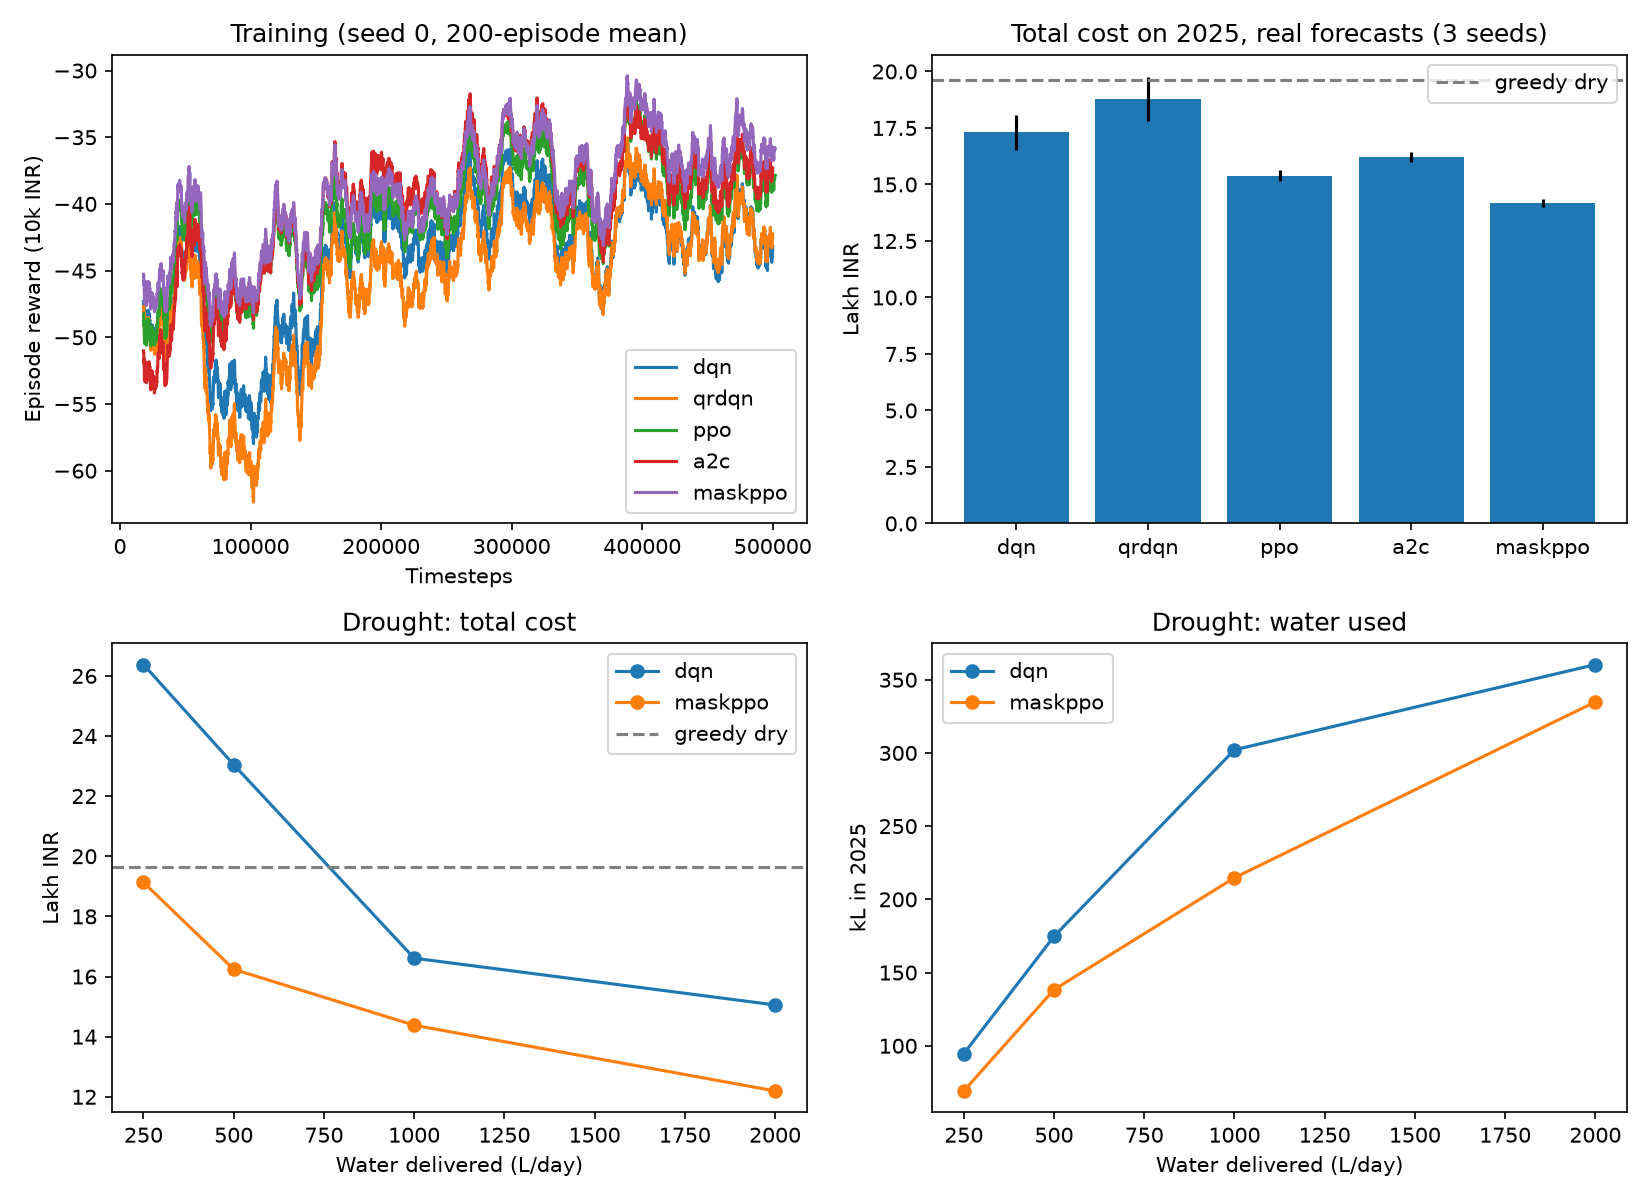
\includegraphics[width=0.49\textwidth,trim=0 0 0 288,clip]{v2/results_v2.png}
\caption{Left: v3 training curves (3 seeds) and 2025 cost against greedy and v2. Right: drought study, MaskablePPO vs DQN (seed 0), 2025 cost and water used as daily water delivery varies.}
\end{figure*}

\textbf{Main result.} The v3 agent costs 13.00 lakh INR on 2025, \textbf{34\% less than greedy}, with 36\% less energy lost, and its 3 seeds agree within 0.04. Every RL method beats greedy.

\textbf{What it learned.} Unlike greedy, the agent spends about 111 days idle, 205 brushing and 48 washing. 96\% of its washes go to blocks holding cemented dust, the only case a brush cannot fix, so water is used where it is irreplaceable.

\begin{figure}[t]
\centering
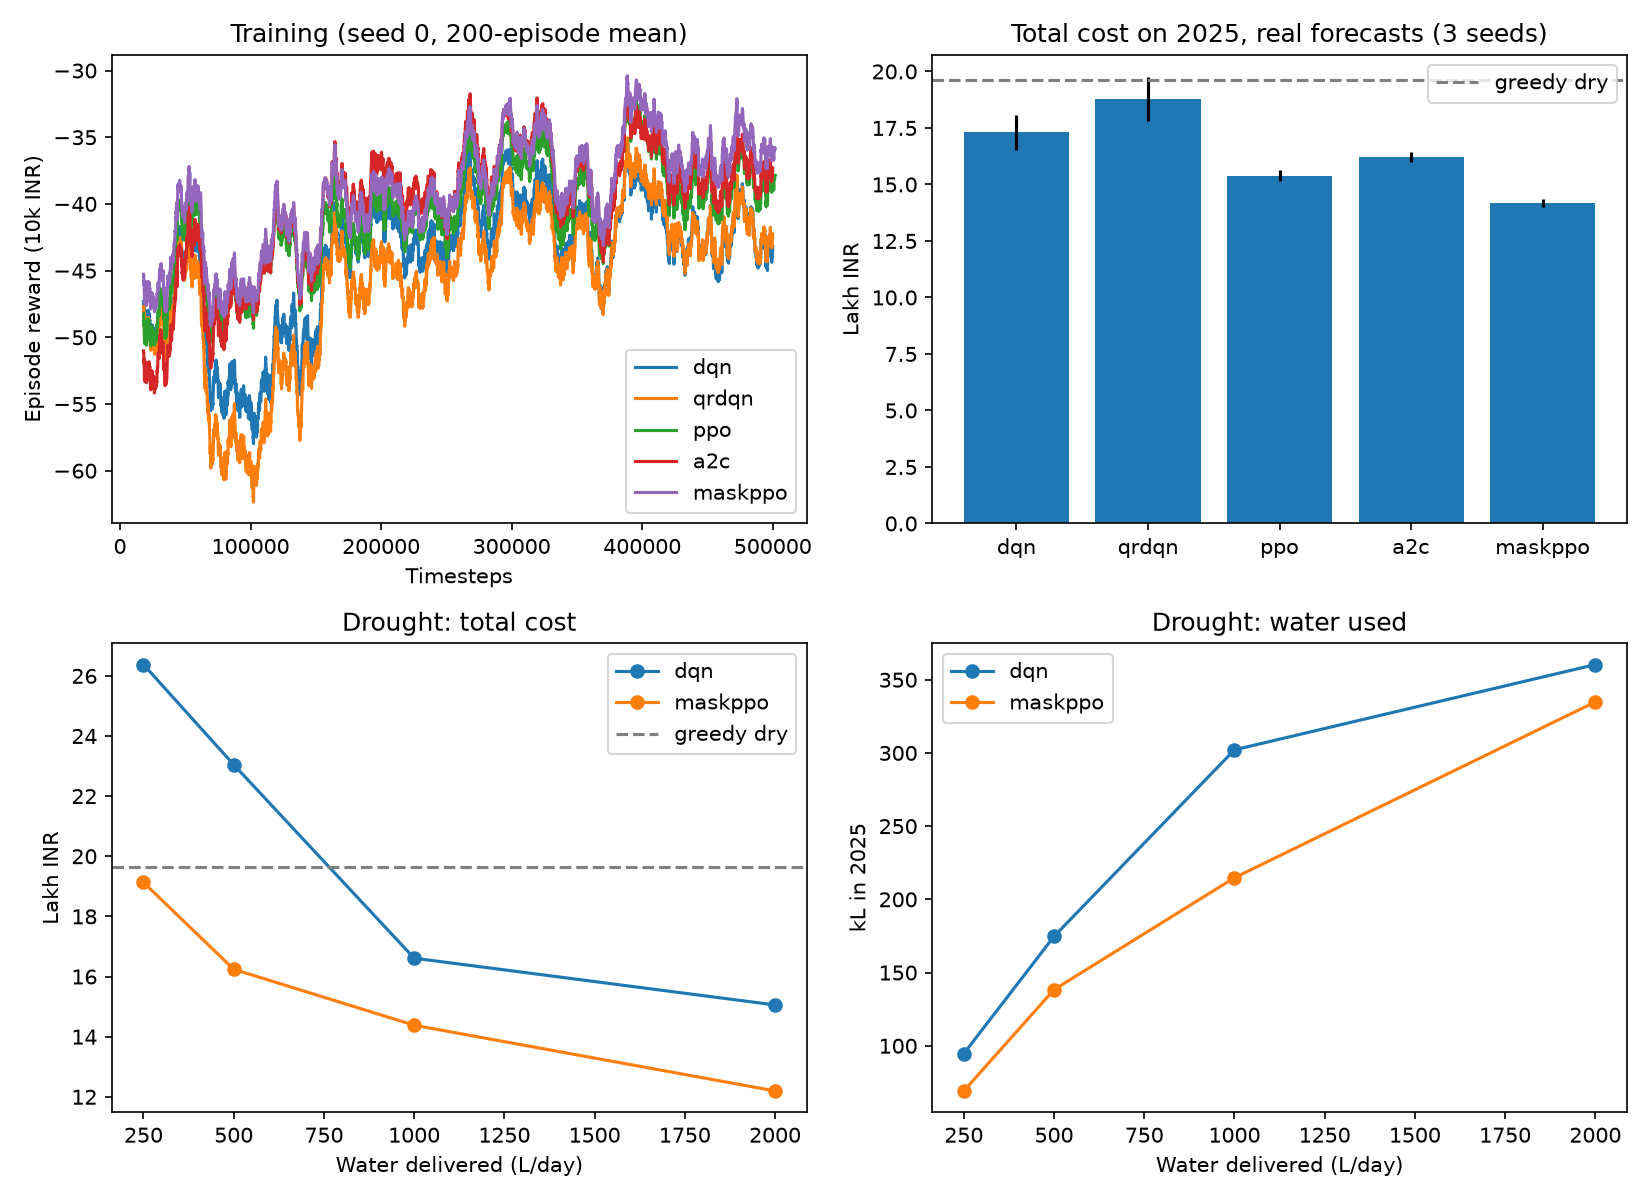
\includegraphics[width=\columnwidth,trim=0 288 0 0,clip]{v2/results_v2.png}
\caption{Algorithm comparison (500k steps, 1,000\,L/day). Left: training reward, seed 0. Right: 2025 cost, 3 seeds; dashed line is greedy.}
\end{figure}

\textbf{On-policy vs value-based.} PPO, A2C and MaskablePPO beat DQN and QR-DQN and vary less across seeds. In validation, DQN also degraded from 500k to 1M steps (2024 cost 22.17$\to$27.19), while MaskablePPO kept improving.

\textbf{Drought study.} With daily water delivery reduced from 2,000 to 250\,L, both agents shift from washing to brushing. Without masking, DQN wastes 166 of 364 crew-days attempting washes with an empty tank and becomes worse than greedy; MaskablePPO stays below greedy at every supply level.

\textbf{Development.} v1 (DQN, perfect forecasts, 18.01) $\to$ v2 (real forecasts, masking, MaskablePPO, 14.18) $\to$ v3 (season, entropy bonus, 13.00); each version subclasses the previous environment.

\textbf{Limitations.} Same-day dust is observed, not forecast; training years before 2024 lack real forecasts; soiling constants come from nearby studies rather than Jaisalmer measurements; and MaskablePPO itself was selected on the 2025 comparison, though v3's additions were selected on 2024 only.

\footnotesize
\begin{thebibliography}{9}\setlength{\itemsep}{0pt}
\bibitem{valerino} M.~Valerino et al., ``Low-cost solar PV soiling sensor validation and size resolved soiling impacts: a comprehensive field study in Western India,'' \emph{Solar Energy} 204, 2020. doi:10.1016/j.solener.2020.03.118
\bibitem{renene} D.~Olivares et al., ``Soiling in the Atacama Desert: impacts on solar performance and evaluation of cleaning techniques,'' \emph{Renewable Energy} 257, 2026. doi:10.1016/j.renene.2025.124815
\bibitem{pvlib} pvlib-python, Kimber soiling model, \url{https://pvlib-python.readthedocs.io}
\bibitem{an} H.~An, ``Reinforcement learning-based dynamic cleaning scheduling framework for solar energy system,'' arXiv:2603.07518, 2026.
\bibitem{terhag} F.~Terhag et al., ``Optimization of cleaning strategies based on ANN algorithms assessing the benefit of soiling rate forecasts,'' \emph{AIP Conf. Proc.} 2126, 220005, 2019.
\bibitem{sb3} A.~Raffin et al., ``Stable-Baselines3: reliable reinforcement learning implementations,'' \emph{JMLR} 22(268), 2021.
\bibitem{maskppo} S.~Huang and S.~Onta\~n\'on, ``A closer look at invalid action masking in policy gradient algorithms,'' \emph{FLAIRS}, 2022.
\end{thebibliography}
\end{document}
